%%%% utfprpgtex.tex, 2018/06/17
%%%% Copyright (C) 2014-2017 Luiz E. M. Lima (luizeduardomlima@gmail.com)
%%
%% Este arquivo pode ser distribuído e/ou modificado sob as condições da
%% Licença Pública do Projeto LaTeX, tanto a versão 1.3 desta licença ou (à sua
%% opção) qualquer versão posterior.
%% A versão mais recente desta licença está disponível em
%%   http://www.latex-project.org/lppl.txt
%% e a versão 1.3 ou posterior faz parte de todas as distribuições de LaTeX
%% versão 2005/12/01 ou posterior.
%%
%% Este arquivo tem o estado de manutenção da LPPL `mantida'.
%%
%% O mantenedor atual deste arquivo é Luiz E. M. Lima.
%%
%% Este projeto consiste dos arquivos utfprpgtex.cls, utfprpgtex.tex e
%% utfprpgtex-dados.tex.
%%
%% utfprpgtex.tex é o arquivo principal do modelo de documento LaTeX para
%% produção de trabalhos acadêmicos da UTFPR.

%% Classe e opções de documento
\documentclass[%% Opções
%% -- Opções da classe memoir --
  12pt,%% Tamanho da fonte: 10pt, 11pt, 12pt, etc.
  a4paper,%% Tamanho do papel: a4paper (A4), letterpaper (carta), etc.
  % fleqn,%% Alinhamento das equações à esquerda (comente para alinhamento centralizado)
  % leqno,%% Numeração das equações no lado esquerdo (comente para lado direito)
  oneside,%% Impressão dos elementos textuais e pós-textuais: oneside (anverso) ou twoside (anverso e verso, se mais de 100 p.)
  openright,%% Impressão da primeira página dos capítulos: openright (anverso), openleft (verso) ou openany (anverso e verso)
%% -- Opções da classe abntex2 --
  sumario = abnt-6027-2012,%% Formatação do sumário: tradicional (estilo tradicional) ou abnt-6027-2012 (norma ABNT 6027-2012)
  chapter = TITLE,%% Títulos de capítulos em maiúsculas (comente para desabilitar)
  section = TITLE,%% Títulos de seções secundárias em maiúsculas (comente para desabilitar)
  % subsection = TITLE,%% Títulos de seções terciárias em maiúsculas (comente para desabilitar)
  % subsubsection = TITLE,%% Títulos de seções quartenárias em maiúsculas (comente para desabilitar)
%% -- Opções da classe utfprpgtex --
  pretextualoneside,%% Impressão dos elementos pré-textuais: pretextualoneside (anverso) ou pretextualtwoside (anverso e verso)
  fontearial,%% Fonte do texto: fontetimes (times), fontearial (arial) ou fontecourier (courier)
  % vinculoscoloridos,%% Cores nos vínculos (citações, arquivos, links, url, etc.) (comente para desabilitar)
  semrecuonosumario,%% Remoção do recuo dos itens no sumário (comente para adição do recuo, se estilo tradicional)
  usemakeindex,%% Compilação de glossários e índices utilizando makeindex (comente para desabilitar)
  % legendascentralizadas,%% Alinhamento das legendas centralizado (comente para alinhamento à esquerda)
  aprovacaoestiloppg,%% Folha de aprovação do programa de pós-graduação no estilo do PPG (comente para estilo padrão)
  pardeassinaturas,%% Assinaturas na folha de aprovação em até duas colunas (comente para em uma única coluna)
  % linhasdeassinaturas,%% Linhas de assinaturas na folha de aprovação (comente para remover as linhas)
%% -- Opções do pacote babel --
  english,%% Idioma adicional para hifenização
  french,%% Idioma adicional para hifenização
  spanish,%% Idioma adicional para hifenização
  brazil,%% Idioma principal do documento (último da lista)
]{utfprpgtex}%% Classe utfprpgtex

%% Pacotes carregados nas classes:
%%   memoir: abstract, appendix, array, booktabs, ccaption, chngcntr, chngpage, dcolumn, delarray, enumerate, epigraph, framed,
%%           ifmtarg, ifpdf, index, makeidx, moreverb, needspace, newfile, nextpage, parskip, patchcmd, setspace, shortvrb, showidx,
%%           tabularx, titleref, titling, tocbibind, tocloft, verbatim, verse.
%%   memoir (similares): crop, fancyhdr, geometry, sidecap, subfigure, titlesec.
%%   abntex2: babel, bookmark, calc, enumitem, ifthen, hyperref, textcase.
%%   utfprpgtex: abntex2cite, ae, algorithmic, amsmath, backref, breakurl, caption, cmap, color, eepic, epic, epsfig, etoolbox,
%%               fancyhdr, fix-cm, fontenc, glossaries, graphics, graphicx, helvet, hyphenat, indentfirst, inputenc, lastpage,
%%               morewrites, nomencl, sfmath, sistyle, substr, times, xtab.

%% Pacotes adicionais (\usepackage[options]{package})
\usepackage{bigdelim, booktabs, colortbl, longtable, multirow}%% Ferramentas para tabelas
\usepackage{amssymb, amstext, amsthm, icomma}%% Ferramentas para linguagem matemática
\usepackage{pifont, textcomp, wasysym}%% Símbolos de texto

%% Comandos personalizados (\newcommand{name}[num]{definition})
\newcommand{\cpp}{\texttt{C$$}}%% C++
\newcommand{\latex}{\LaTeX}%% LaTeX
\newcommand{\ds}{\displaystyle}%% Tamanho normal das equações
\newcommand{\bsym}[1]{\boldsymbol{#1}}%% Texto no modo matemático em negrito
\newcommand{\mr}[1]{\mathrm{#1}}%% Texto no modo matemático normal (não itálico)
\newcommand{\der}{\mr{d}}%% Operador diferencial
\newcommand{\deri}[2]{\frac{\der #1}{\der #2}}%% Derivada ordinária
\newcommand{\derip}[2]{\frac{\partial #1}{\partial #2}}%% Derivada parcial
\newcommand{\pare}[1]{\left( #1 \right)}%% Parênteses
\newcommand{\colc}[1]{\left[ #1 \right]}%% Colchetes
\newcommand{\chav}[1]{\left\lbrace #1 \right\rbrace}%% Chaves
\newcommand{\sen}{\operatorname{sen}}%% Operador seno
\newcommand{\senh}{\operatorname{senh}}%% Operador seno hiperbólico
\newcommand{\tg}{\operatorname{tg}}%% Operador tangente
\newcommand{\tgh}{\operatorname{tgh}}%% Operador tangente hiperbólico
\newcommand{\seqref}[1]{Equação~\eqref{#1}}%% Referência de uma única equação
\newcommand{\meqref}[1]{Equações~\eqref{#1}}%% Referência de multiplas equações
\newcommand{\citep}[1]{\cite{#1}}%% Atalho para citação implícita
\newcommand{\citet}[1]{\citeonline{#1}}%% Atalho para citação explícita
\newcommand{\citepa}[1]{(\citeauthor{#1})}%% Atalho para citação implícita (somente autor)
\newcommand{\citeta}[1]{\citeauthoronline{#1}}%% Atalho para citação explícita (somente autor)
\newcommand{\citepy}[1]{(\citeyear{#1})}%% Atalho para citação implícita (somente ano)
\newcommand{\citety}[1]{\citeyear{#1}}%% Atalho para citação explícita (somente ano)

%% Arquivo de dados do modelo de documento LaTeX para produção de trabalhos acadêmicos da UTFPR
%%%% utfprpgtex-dados.tex, 2018/06/17
%%%% Copyright (C) 2014-2017 Luiz E. M. Lima (luizeduardomlima@gmail.com)
%%
%% Este arquivo pode ser distribuído e/ou modificado sob as condições da
%% Licença Pública do Projeto LaTeX, tanto a versão 1.3 desta licença ou (à sua
%% opção) qualquer versão posterior.
%% A versão mais recente desta licença está disponível em
%%   http://www.latex-project.org/lppl.txt
%% e a versão 1.3 ou posterior faz parte de todas as distribuições de LaTeX
%% versão 2005/12/01 ou posterior.
%%
%% Este arquivo tem o estado de manutenção da LPPL `mantida'.
%%
%% O mantenedor atual deste arquivo é Luiz E. M. Lima.
%%
%% Este projeto consiste dos arquivos utfprpgtex.cls, utfprpgtex.tex e
%% utfprpgtex-dados.tex.
%%
%% utfprpgtex-dados.tex é o arquivo de dados do modelo de documento LaTeX para
%% produção de trabalhos acadêmicos da UTFPR.

%% Documento
\TipoDeDocumento{Tese}%% Tipo de documento: "Tese", "Dissertação" ou "Trabalho de Conclusão de Curso"
\DocumentType{Thesis}%% Document type: "Thesis", "Dissertation" ou "Final Coursework"
\NivelDeFormacao{Doutorado}%% Nível de formação: "Doutorado", "Mestrado" ou "Bacharelado"
\FormationLevel{Doctorate}%% Formation level: "Doctorate", "Master's Degree" ou "Bachelor's Degree"
\TituloDoDocumento{%% Título do documento
  Título do presente trabalho acadêmico: subtítulo do presente trabalho acadêmico
}
\DocumentTitle{%% Document title
  Title of this academic work: subtitle of this academic work
}
\TituloEmMultiplasLinhas{%% Título em multiplas linhas na capa e nas folhas de rosto e de aprovação (\par indica a quebra de linha)
  Título do presente trabalho acadêmico: \par subtítulo do presente trabalho acadêmico
}
\DescricaoDoDocumento{%% Descrição do documento na folha de rosto
  \imprimirtipodedocumento\ apresentado(a) como requisito parcial à obtenção do título de \imprimirtitulopretendido\ em
  \imprimircurso, do \imprimirppgoudepartamento, da \imprimirinstituicao.
}
\TituloDaFichaCatalografica{%% Título da ficha catalográfica
  Ficha catalográfica elaborada pelo Departamento de Biblioteca da \par \imprimirinstituicao, Câmpus \imprimircidade \par n.
  \imprimirnumerodapublicacao
}
\TextoDeAprovacao{%% Texto de aprovação
  %% Exemplo de texto de aprovação para Tese ou Dissertação (descomente a próxima linha para utilizá-lo):
  Esta \imprimirtipodedocumento\ foi apresentada às 00:00 de \imprimirdia\ de \imprimirmesporextenso\ de \imprimirano\ como requisito parcial para a obtenção do título de \imprimirtitulopretendido\ em \imprimircurso, na área de concentração em \imprimirareadeconcentracao\ e na linha de pesquisa em (Nome da Linha de Pesquisa), do Programa de Pós-Graduação em \imprimircurso. O(A) candidato(a) foi arguido(a) pela Banca Examinadora composta pelos professores abaixo citados. Após deliberação, a Banca Examinadora considerou o trabalho aprovado.
  %% Exemplo de texto de aprovação para Trabalho de Conclusão de Curso (descomente a próxima linha para utilizá-lo):
  % Este \imprimirtipodedocumento\ foi apresentado em \imprimirdia\ de \imprimirmesporextenso\ de \imprimirano\ como requisito parcial para a obtenção do título de \imprimirtitulopretendido\ em \imprimircurso. O(A) candidato(a) foi arguido(a) pela Banca Examinadora composta pelos professores abaixo assinados. Após deliberação, a Banca Examinadora considerou o trabalho aprovado.
}
\AvisoDeAprovacao{%% Aviso de aprovação
  %% Exemplo de aviso de aprovação para Tese ou Dissertação (descomente a próxima linha para utilizá-lo):
  A Folha de Aprovação assinada encontra-se no \par Departamento de Registros Acadêmicos da UTFPR -- Câmpus \imprimircidade
  %% Exemplo de aviso de aprovação para Trabalho de Conclusão de Curso (descomente a próxima linha para utilizá-lo):
  % -- O Termo de Aprovação assinado encontra-se na Coordenação do Curso --
}
\NumeroDaTeseOuDissertacao{00/\imprimirano}%% Número da Tese ou Dissertação - Fornecido pelo programa de pós-graduação
\NumeroDaPublicacao{00/\imprimirano}%% Número da publicação - Fornecido pela biblioteca
\NumeroDaFichaCatalografica{A000}%% Número da ficha catalográfica - Fornecido pela biblioteca
\CDDOuCDU{CDD 000.00}%% Classificação Decimal Dewey (CDD) ou Classificação Decimal Universal (CDU) - Fornecida pela biblioteca

%% Autor(a)
\TituloPretendido{Doutor(a)}%% Título pretendido: "Doutor(a)", "Mestre(a)" ou "Bacharel(a)"
\NomeDoAutor{Nome do(a) Autor(a)}%% Nome completo do(a) autor(a)
\SobrenomeDoAutor{Último Nome}%% Último nome do(a) autor(a)
\PrenomeDoAutor{Resto do Nome do(a) Autor(a)}%% Nome do(a) autor(a) sem último nome

%% Outro(a) autor(a) (Trabalho de Conclusão de Curso)
\AtribuiOutroAutor{true}%% Insere ou remove outro(a) autor(a): "true" ou "false"
\NomeDoOutroAutor{Nome do(a) Outro(a) Autor(a)}%% Nome completo do(a) outro(a) autor(a)
\SobrenomeDoOutroAutor{Último Nome}%% Último nome do(a) outro(a) autor(a)
\PrenomeDoOutroAutor{Resto do Nome do(a) Outro(a) Autor(a)}%% Nome do(a) outro(a) autor(a) sem último nome

%% Orientador(a)
\AtribuicaoOrientador{Orientador(a)}%% Atribuição "Orientador(a)"
\TituloDoOrientador{Prof(a). Dr(a).}%% Título do(a) orientador(a)
\NomeDoOrientador{Nome do(a) Orientador(a)}%% Nome completo do(a) orientador(a)
\SobrenomeDoOrienador{Último Nome}%% Último nome do(a) orientador(a)
\PrenomeDoOrientador{Resto do Nome do(a) Orientador(a)}%% Nome do(a) orientador(a) sem último nome

%% Coorientador(a)
\AtribuiCoorientador{true}%% Insere ou remove o(a) coorientador(a): "true" ou "false"
\AtribuicaoCoorientador{Coorientador(a)}%% Atribuição "Coorientador(a)"
\TituloDoCoorientador{Prof(a). Dr(a).}%% Título do(a) coorientador(a)
\NomeDoCoorientador{Nome do(a) Coorientador(a)}%% Nome completo do(a) coorientador(a)
\SobrenomeDoCoorienador{Último Nome}%% Último nome do(a) coorientador(a)
\PrenomeDoCoorientador{Resto do Nome do(a) Coorientador(a)}%% Nome do(a) coorientador(a) sem último nome

%% Instituição
\Instituicao{Universidade Tecnológica Federal do Paraná}%% Nome da instituição
\Institution{Federal University of Technology -- Paraná}%% Institution name
\Cidade{Ponta Grossa}%% Nome da cidade (câmpus)
\Diretoria{Pesquisa e Pós-Graduação}%% Diretoria: "Graduação e Educação Profissional" ou "Pesquisa e Pós-Graduação"
\Departamento{Nome do Departamento ou da Coordenação}%% Nome do departamento ou da coordenação
\Curso{Nome do Curso}%% Nome do curso
\Course{Course Name}%% Course name
\AreaDeConcentracao{Nome da Área de Concentração}%% Nome da área de concentração
\TituloDoResponsavelTCC{Prof(a). Dr(a).}%% Título do(a) responsável pelos TCC
\NomeDoResponsavelTCC{Nome do(a) Responsável}%% Nome completo do(a) responsável pelos TCC
\AtribuicaoCoordenador{Coordenador(a)}%% Atribuição "Coordenador(a)" do curso
\TituloDoCoordenador{Prof(a). Dr(a).}%% Título do(a) coordenador(a) do curso
\NomeDoCoordenador{Nome do(a) Coordenador(a)}%% Nome completo do(a) coordenador(a) do curso
\SiglaDoPPG{PPG}%% Sigla do programa de pós-graduação: PPGBIOTEC, PPGCC, PPGECT, PPGEE, PPGEM, PPGEP ou PPGEQ

%% Banca examinadora: 3 membros (Trabalho de Conclusão de Curso ou Dissertação); 5 a 7 membros (Tese)
\MembroAIgualOrientador{true}%% Insere ou remove o membro A igual ao(à) orientador(a): "true" ou "false"
\MembroA{Nome do Membro A}%% Nome completo do membro A - Presidente (automático se orientador(a))
\TituloDoMembroA{Prof(a). Dr(a).}%% Título do membro A - Presidente (automático se orientador(a))
\InstituicaoDoMembroA{Instituição do Membro A}%% Nome da instituição do membro A - Presidente (automático se orientador(a))
\MembroB{Nome do Membro B}%% Nome completo do membro B
\TituloDoMembroB{Prof(a). Dr(a).}%% Título do membro B
\InstituicaoDoMembroB{Instituição do Membro B}%% Nome da instituição do membro B
\MembroC{Nome do Membro C}%% Nome completo do membro C
\TituloDoMembroC{Prof(a). Dr(a).}%% Título do membro C
\InstituicaoDoMembroC{Instituição do Membro C}%% Nome da instituição do membro C
\MembroD{Nome do Membro D}%% Nome completo do membro D
\TituloDoMembroD{Prof(a). Dr(a).}%% Título do membro D
\InstituicaoDoMembroD{Instituição do Membro D}%% Nome da instituição do membro D
\MembroE{Nome do Membro E}%% Nome completo do membro E
\TituloDoMembroE{Prof(a). Dr(a).}%% Título do membro E
\InstituicaoDoMembroE{Instituição do Membro E}%% Nome da instituição do membro E
\AtribuiMembroF{false}%% Insere ou remove o Membro F: "true" ou "false"
\MembroF{Nome do Membro F}%% Nome completo do membro F
\TituloDoMembroF{Prof(a). Dr(a).}%% Título do membro F
\InstituicaoDoMembroF{Instituição do Membro F}%% Nome da instituição do membro F
\AtribuiMembroG{false}%% Insere ou remove o Membro G: "true" ou "false"
\MembroG{Nome do Membro G}%% Nome completo do membro G
\TituloDoMembroG{Prof(a). Dr(a).}%% Título do membro G
\InstituicaoDoMembroG{Instituição do Membro G}%% Nome da instituição do membro G

%% Data da defesa
\Dia{1}%% Dia
\MesPorExtenso{janeiro}%% Mês por extenso
\Ano{2015}%% Ano

%% Palavras-chave e keywords
\NumeroDePalavrasChave{5}%% Número de palavras-chave (máximo 5)
\PalavraChaveA{Palavra-chave A}%% Palavra-chave A
\PalavraChaveB{Palavra-chave B}%% Palavra-chave B
\PalavraChaveC{Palavra-chave C}%% Palavra-chave C
\PalavraChaveD{Palavra-chave D}%% Palavra-chave D
\PalavraChaveE{Palavra-chave E}%% Palavra-chave E
\NumeroDeKeywords{5}%% Número de keywords (máximo 5)
\KeywordA{Keyword A}%% Keyword A
\KeywordB{Keyword B}%% Keyword B
\KeywordC{Keyword C}%% Keyword C
\KeywordD{Keyword D}%% Keyword D
\KeywordE{Keyword E}%% Keyword E
%% Realize as modificações pertinentes no arquivo "utfprpgtex-dados.tex"

%% Ferramenta para criação de índices
\makeindex%% Não comente esta linha

%% Ferramenta para criação de glossários
\makeglossaries%% Não comente esta linha
%%%% LISTA DE ABREVIATURAS, SIGLAS E ACRÔNIMOS
%%
%% Relação, em ordem alfabética, das abreviaturas (representação de uma palavra por meio de alguma(s) de sua(s) sílaba(s) ou
%% letra(s)), siglas (conjunto de letras iniciais dos vocábulos e/ou números que representa um determinado nome) e acrônimos
%% (conjunto de letras iniciais dos vocábulos e/ou números que representa um determinado nome, formando uma palavra pronunciável).
%%
%% Este arquivo para definição de abreviaturas, siglas e acrônimos é utilizado com a opção "glossaries" (pacote)

%% Abreviaturas: \abreviatura{rótulo}{representação}{definição}

\abreviatura{art.}{art.}{Artigo}
\abreviatura{cap.}{cap.}{Capítulo}
\abreviatura{sec.}{sec.}{Seção}

%% Siglas: \sigla{rótulo}{representação}{definição}

\sigla{abnt}{ABNT}{Associação Brasileira de Normas Técnicas}
\sigla{cnpq}{CNPq}{Conselho Nacional de Desenvolvimento Científico e Tecnológico}
\sigla{eps}{EPS}{\textit{Encapsulated PostScript}}
\sigla{pdf}{PDF}{Formato de Documento Portátil, do inglês \textit{Portable Document Format}}
\sigla{ps}{PS}{\textit{PostScript}}
\sigla{utfpr}{UTFPR}{Universidade Tecnológica Federal do Paraná}

%% Acrônimos: \acronimo{rótulo}{representação}{definição}

\acronimo{gimp}{Gimp}{Programa de Manipulação de Imagem GNU, do inglês \textit{GNU Image Manipulation Program}}
%% Entradas da lista de abreviaturas, siglas e acrônimos - Comente para remover este item
%%%% GLOSSÁRIO
%%
%% Relação de palavras ou expressões técnicas de uso restrito ou de sentido obscuro, utilizadas no texto, acompanhadas das
%% respectivas definições.

%% Entradas do glossário: \newglossaryentry{rótulo}{informações da entrada}

\newglossaryentry{pai}{%% Informações da entrada
  name        = {pai},
  plural      = {pais},
  description = {um exemplo de entrada pai que possui subentradas (entradas filhas)}
}

\newglossaryentry{componente}{%% Informações da entrada
  name        = {componente},
  plural      = {componentes},
  parent      = {pai},
  description = {um exemplo de uma entrada componente, subentrada da entrada chamada \gls{pai}}
}

\newglossaryentry{filho}{%% Informações da entrada
  name        = {filho},
  plural      = {filhos},
  parent      = {pai},
  description = {um exemplo de uma entrada filha (subentrada) da entrada chamada \gls{pai}. Trata-se de uma entrada irmã da entrada chamada \gls{componente}}
}

\newglossaryentry{equilibrio}{%% Informações da entrada
  name        = {equilíbrio da configuração},
  see         = [veja também]{componente},
  description = {uma consistência entre os \glspl{componente}}
}

\newglossaryentry{tex}{%% Informações da entrada
  name        = {\TeX},
  sort        = {TeX},
  description = {é um sistema de tipografia criado por Donald E. Knuth}
}

\newglossaryentry{latex}{%% Informações da entrada
  name        = {\latex},
  sort        = {LaTeX},
  description = {um conjunto de macros para o processador de textos \gls{tex}, utilizado amplamente para a produção de textos matemáticos e científicos devido à sua alta qualidade tipográfica}
}

\newglossaryentry{bibtex}{%% Informações da entrada
  name        = {Bib\TeX},
  sort        = {BibTeX},
  parent      = {latex},
  description = {um software de gerenciamento de referências para a formatação de listas de referências. A ferramenta Bib\TeX\ é normalmente usada em conjunto com o sistema de preparação de documentos do \gls{latex}}
}

\newglossaryentry{abntex2}{%% Informações da entrada
  name        = {\abnTeX},
  sort        = {abnTeX2},
  see         = {latex},
  description = {uma suíte para \gls{latex} que atende os requisitos das normas da Associação Brasileira de Normas Técnicas (ABNT) para elaboração de documentos técnicos e científicos brasileiros, como artigos científicos, relatórios técnicos, trabalhos acadêmicos como teses, dissertações, projetos de pesquisa e outros documentos do gênero}
}

\newglossaryentry{utfprpgtex}{%% Informações da entrada
  name        = {\utfprpgtex},
  sort        = {UTFPRPGTeX},
  see         = {latex},
  parent      = {abntex2},
  description = {uma suíte para \gls{latex}, baseada na suíte \gls{abntex2}, que atende os requisitos das normas definidas pela Universidade Tecnológica Federal do Paraná (UTFPR), câmpus Ponta Grossa, para elaboração de trabalhos acadêmicos}
}
%% Entradas do glossário - Comente para remover este item

%% Ferramenta para criação de nomenclaturas
\makenomenclature%% Não comente esta linha

%% Início do documento
\begin{document}%% Não comente esta linha

%% Formatação de páginas de elementos pré-textuais
\pretextual%% Não comente esta linha

%% Capa
\incluircapa%% Comente para remover este item

%% Folha de rosto (* coloca a ficha bibliográfica no verso)
\incluirfolhaderosto*%% Comente para remover este item

%% Ficha catalográfica (teses e dissertações)
%%\incluirfichacatalografica%% Comente para remover este item

%% Errata
%%%%%% ERRATA
%%
%% Lista dos erros ocorridos no texto, seguidos das devidas correções.

\begin{errata}%% Ambiente errata
\begin{table*}[htb]%% Ambiente table
\begin{tabularx}{\textwidth}{|l|l|X|X|}%% Ambiente tabularx
\hline
\textbf{Página(s)}         & \textbf{Linha(s)} & \textbf{Onde se lê} & \textbf{Leia-se}         \\ \hline
\pageref*{errata:capitulo} & 4, 9-11, 14-16    & capítulo(s)         & seção(ões) primária(s)   \\ \hline
\pageref*{errata:secao}    & 12-16             & seção(ões)          & seção(ões) secundária(s) \\ \hline
\pageref*{errata:subsecao} & 16                & subseção(ões)       & seção(ões) terciária(s)  \\ \hline
\end{tabularx}
\end{table*}
\end{errata}
%% Comente para remover este item

%% Folha de aprovação
\incluirfolhadeaprovacao%% Comente para remover este item

%% Dedicatória
%%%% DEDICATÓRIA
%%
%% Texto em que o autor presta homenagem ou dedica seu trabalho.

\begin{dedicatoria}%% Ambiente dedicatoria
Dedico este trabalho a minha família e aos meus amigos, pelos momentos de ausência.
\end{dedicatoria}
%% Comente para remover este item

%% Agradecimentos
%%%% AGRADECIMENTOS
%%
%% Texto em que o autor faz agradecimentos dirigidos àqueles que contribuíram de maneira relevante à elaboração do trabalho.

\begin{agradecimentos}%% Ambiente agradecimentos
Este trabalho não poderia ser terminado sem a ajuda de diversas pessoas e/ou instituições às quais presto minha homenagem. Certamente esses parágrafos não irão atender a todas as pessoas que fizeram parte dessa importante fase de minha vida. Portanto, desde já peço desculpas àquelas que não estão presentes entre estas palavras, mas elas podem estar certas que fazem parte do meu pensamento e de minha gratidão.

A minha família, pelo carinho, incentivo e total apoio em todos os momentos da minha vida.

Ao meu orientador, que me mostrou os caminhos a serem seguidos e pela confiança depositada.

A todos os professores e colegas do departamento, que ajudaram de forma direta e indireta na conclusão deste trabalho.

Ao \gls{cnpq}, pelo apoio financeiro.

Enfim, a todos os que de alguma forma contribuíram para a realização deste trabalho.
\end{agradecimentos}
%% Comente para remover este item

%% Epígrafe
%%%% EPÍGRAFE
%%
%% Texto em que o autor apresenta uma citação, seguida de indicação de autoria, relacionada com a matéria tratada no corpo do
%% trabalho.

\begin{epigrafe}%% Ambiente epigrafe
Primeira Lei: Um robô não pode ferir um ser humano ou, por omissão, permitir que um ser humano sofra algum mal. Segunda Lei: Um robô deve obedecer as ordens que lhe sejam dadas por seres humanos, exceto nos casos em que tais ordens contrariem a Primeira Lei. Terceira Lei: Um robô deve proteger sua própria existência desde que tal proteção não entre em conflito com a Primeira e Segunda Leis (ASIMOV, Isaac, 1950).
\end{epigrafe}
%% Comente para remover este item

%% Resumo
%%%% RESUMO
%%
%% Apresentação concisa dos pontos relevantes de um texto, fornecendo uma visão rápida e clara do conteúdo e das conclusões do
%% trabalho.

\begin{resumoutfpr}%% Ambiente resumoutfpr
O resumo deve ser redigido na terceira pessoa do singular, com verbo na voz ativa, não ultrapassando uma página (de 150 a 500 palavras, segundo a ABNT NBR 6028), evitando-se o uso de parágrafos no meio do resumo, assim como fórmulas, equações e símbolos. Iniciar o resumo situando o trabalho no contexto geral, apresentar os objetivos, descrever a metodologia adotada, relatar a contribuição própria, comentar os resultados obtidos e finalmente apresentar as conclusões mais importantes do trabalho. As palavras-chave devem aparecer logo abaixo do resumo, antecedidas da expressão Palavras-chave. Para definição das palavras-chave (e suas correspondentes em inglês no \textit{abstract}) consultar em Termo tópico do Catálogo de Autoridades da Biblioteca Nacional, disponível em: \url{http://acervo.bn.br/sophia_web/index.html}.
\end{resumoutfpr}
%% Comente para remover este item

%% Abstract
%%%% ABSTRACT
%%
%% Versão do resumo para idioma de divulgação internacional.

\begin{abstractutfpr}%% Ambiente abstractutfpr
The abstract should be drafted in the third person singular with the verb in the active voice, not exceeding one page (from 150 to 500 words, according to ABNT NBR 6028), avoiding the use of paragraphs in the middle of the summary, formulas, equations and symbols. Start the abstract setting the work in the general context, presenting the objectives, describe the methodology adopted, reporting the contribution itself, commenting on the results and finally present the conclusions of the most important work. The keywords should appear below the abstract, preceded by the expression Keywords. To define the keywords (and their corresponding portuguese in the \textit{resumo}) query in Authorities Catalog Topic term of the National Library, available at: \url{http://acervo.bn.br/sophia_web/index.html}.
\end{abstractutfpr}
%% Comente para remover este item

%% Lista de algoritmos
\incluirlistadealgoritmos%% Comente para remover este item

%% Lista de ilustrações
\incluirlistadeilustracoes%% Comente para remover este item

%% Lista de tabelas
\incluirlistadetabelas%% Comente para remover este item

%% Lista de abreviaturas, siglas e acrônimos
\incluirlistadeacronimos{glossaries}%% Opções: "glossaries" (pacote) ou "file" (arquivo) ou "none" (desabilita)

%% Lista de símbolos
\incluirlistadesimbolos{nomencl}%% Opções: "nomencl" (pacote) ou "file" (arquivo) ou "none" (desabilita)

%% Sumário
\incluirsumario%% Comente para remover este item

%% Formatação de páginas de elementos textuais
\textual%% Não comente esta linha

%% Parte
% \part{Introdução}%% Comente para remover este item

%% Capítulo

%% Capítulo de exemplo
% Options for packages loaded elsewhere
\PassOptionsToPackage{unicode}{hyperref}
\PassOptionsToPackage{hyphens}{url}
%
\documentclass[
]{article}
\usepackage{lmodern}
\usepackage{amssymb,amsmath}
\usepackage{ifxetex,ifluatex}
\ifnum 0\ifxetex 1\fi\ifluatex 1\fi=0 % if pdftex
  \usepackage[T1]{fontenc}
  \usepackage[utf8]{inputenc}
  \usepackage{textcomp} % provide euro and other symbols
\else % if luatex or xetex
  \usepackage{unicode-math}
  \defaultfontfeatures{Scale=MatchLowercase}
  \defaultfontfeatures[\rmfamily]{Ligatures=TeX,Scale=1}
\fi
% Use upquote if available, for straight quotes in verbatim environments
\IfFileExists{upquote.sty}{\usepackage{upquote}}{}
\IfFileExists{microtype.sty}{% use microtype if available
  \usepackage[]{microtype}
  \UseMicrotypeSet[protrusion]{basicmath} % disable protrusion for tt fonts
}{}
\makeatletter
\@ifundefined{KOMAClassName}{% if non-KOMA class
  \IfFileExists{parskip.sty}{%
    \usepackage{parskip}
  }{% else
    \setlength{\parindent}{0pt}
    \setlength{\parskip}{6pt plus 2pt minus 1pt}}
}{% if KOMA class
  \KOMAoptions{parskip=half}}
\makeatother
\usepackage{xcolor}
\IfFileExists{xurl.sty}{\usepackage{xurl}}{} % add URL line breaks if available
\IfFileExists{bookmark.sty}{\usepackage{bookmark}}{\usepackage{hyperref}}
\hypersetup{
  hidelinks,
  pdfcreator={LaTeX via pandoc}}
\urlstyle{same} % disable monospaced font for URLs
\usepackage{graphicx,grffile}
\makeatletter
\def\maxwidth{\ifdim\Gin@nat@width>\linewidth\linewidth\else\Gin@nat@width\fi}
\def\maxheight{\ifdim\Gin@nat@height>\textheight\textheight\else\Gin@nat@height\fi}
\makeatother
% Scale images if necessary, so that they will not overflow the page
% margins by default, and it is still possible to overwrite the defaults
% using explicit options in \includegraphics[width, height, ...]{}
\setkeys{Gin}{width=\maxwidth,height=\maxheight,keepaspectratio}
% Set default figure placement to htbp
\makeatletter
\def\fps@figure{htbp}
\makeatother
\setlength{\emergencystretch}{3em} % prevent overfull lines
\providecommand{\tightlist}{%
  \setlength{\itemsep}{0pt}\setlength{\parskip}{0pt}}
\setcounter{secnumdepth}{-\maxdimen} % remove section numbering

\date{}

\begin{document}

\begin{enumerate}
\def\labelenumi{\arabic{enumi}.}
\setcounter{enumi}{2}
\tightlist
\item
  Abrir gerações
\end{enumerate}

Abrir geracoes junto com a matriz energetica

\hypertarget{introduuxe7uxe3o}{%
\section{Introdução}\label{introduuxe7uxe3o}}

Desde seus tempos mais remotos o homem busca soluções de facilitar sua
vida e seu esforço. seja por meio do uso de sistemas mecânicos ou até
mesmo recorrendo às forças de animais. Descoberta em meados do século
XVIII, por Benjamin Franklin\footnote{http://www.ifsc.usp.br/\textasciitilde cibelle/arquivos/T0150-1.pdf},
a eletricidade é sem sombra de dúvidas um grande avanço para a
incansável procura pela comodidade humana. Desde então a ciência está
sempre investigando formas de automatizar trabalhos complexos e
demorados com o uso de circuitos.

A geração de energia é um assunto muito pesquisado para os dias atuais.
Um motivo dessas pesquisas é o constante aumento de energia demandada,
seja para atividades domésticas ou serviços industriais. Para tais
problemas a eletrônica de potência tem grande colaboração na redução de
energia demandada, visando sempre o processamento eletrônico de energia,
causando maiores eficiências em circuitos, redução de volume e peso de
componentes, para que de tal forma a energia requerida pela população
seja menor.

Mesmo com a capacidade de geração de energia presente, em muitos lugares
a entrega de energia acaba sendo comprometida, seja pelas distâncias
entre subestações, ou até mesmo por eventuais faltas de sistemas
apropriados para uma eficiente distribuição. Em alguns casos até
mudanças climáticas acarretam em acidentes e imprevistos com o
fornecimento de energia, causando contratempos tanto para os
consumidores quanto para as próprias concessionárias.

Ao se fazer o projeto de uma usina, são feitos todos os levantamentos
referentes aos seus custos de instauração, licenciamento e
retorno.\footnote{https://www.hidroenergia.com.br/veja-quais-sao-as-etapas-para-construcao-de-uma-hidreletrica/}
Esses levantamentos ocasionalmente concluem que pode não ser possível
para a empresa a construção desse projeto, o que leva a um fornecimento
de energia debilitado até alguns clientes. Outro ponto refletido ao se
construir uma usina são os danos que provocados ao redor de sua
construção, danos os quais podem ser na parte ambiental, como o
desmatamento, a perfuração do solo, a inundação de lugares; ou até mesmo
sociais, como a isolação de terrenos para segurança da região ao redor
ou o ruído incômodo que será provocado. Esses pontos são também
problemas levados em consideração quando uma empresa quer construir uma
usina de grande porte.

Para tais problemas se faz importante o estudo completo de fontes de
geração e conversão de energia, seus custos, impactos e benefícios em
relação as outras formas. Do mesmo modo é necessário compreender as
naturezas de produção de energia e a matriz energética nacional e
mundial.

\hypertarget{matriz-energuxe9tica-atual}{%
\section{Matriz energética atual}\label{matriz-energuxe9tica-atual}}

A geração de energia no Brasil é em sua maior parte hidráulica, o que
não é ruim, pois a água é uma fonte renovável de energia, entretanto há
danos que são causados com a criação de usinas, como a inundação de uma
grande região, causando danos às pessoas que ficam desabrigadas, sem
contar à fauna e à flora. Entretanto, no mundo, a situação é outra: a
maior parte da energia mundial em cenário global é feita a base de
carvão mineral, uma matéria prima que não é renovável e difícil de ser
retirada do meio ambiente.

\hypertarget{sec:matriz_br}{%
\subsection{Brasil}\label{sec:matriz_br}}

Por mais que atualmente a maior parte da geração da energia elétrica
brasileira seja com base na água, é possível destacar um grande aumento
e incentivos(seja pelo governo ou pelos movimentos ambientais) de
gerações alternativas, como gás natural, biomassa e eólica. Este fato
pode ser observado na comparação dentre as figuras
{[}-@fig:brasil\_73{]} e {[}-@fig:brasil\_18{]} a seguir. Em 1999, a
maior parte da eletricidade provinha de hidrelétricas ao Brasil. Já em
2018, pôde-se notar uma grande mudança no cenário energético nacional.

\begin{figure}
\hypertarget{fig:brasil_73}{%
\centering
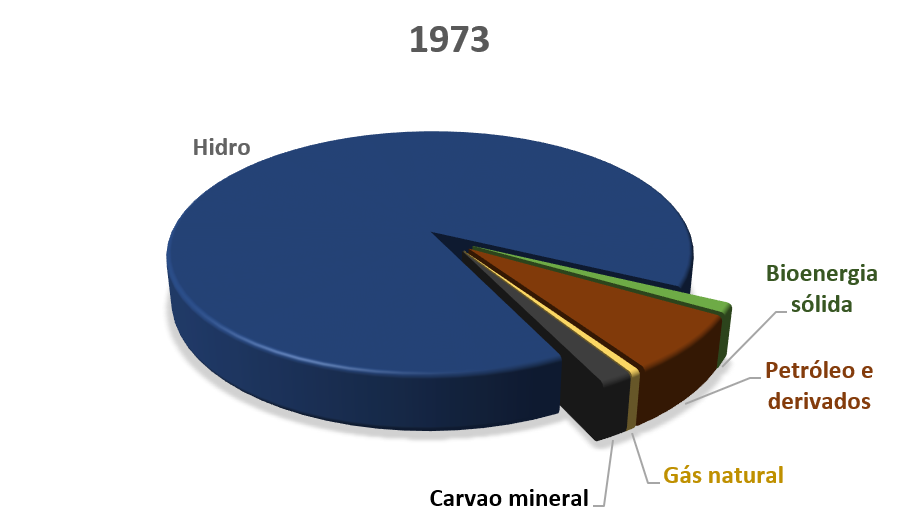
\includegraphics[width=3.125in,height=\textheight]{img/matriz/brasil_73.png}
\caption{Matriz elétrica brasileira - 1973, Fonte: MME, Autoria
própria}\label{fig:brasil_73}
}
\end{figure}

\begin{figure}
\hypertarget{fig:brasil_18}{%
\centering
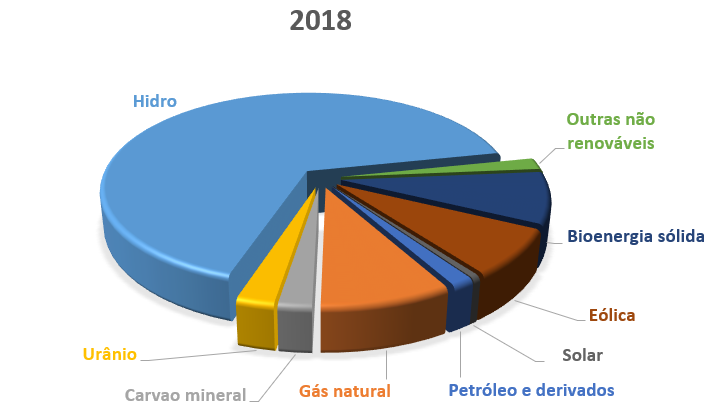
\includegraphics[width=3.125in,height=\textheight]{img/matriz/brasil_18.png}
\caption{Matriz elétrica brasileira - 2018, Fonte: MME, Autoria
própria}\label{fig:brasil_18}
}
\end{figure}

Também é perceptível o aumento da participação da geração de carvão
mineral, de 1.7\% a 2.2\%. Por mais que pareça ter aumentado em 0.5
pontos percentuais, na verdade a geração mineral brasileira serve para
cobrir faltas da geração hidráulica as quais não conseguem ser entregues
quando há períodos de secas, causadora do baixo nível nos reservatórios
das represas.\footnote{http://www.mme.gov.br/documents/1138787/1732840/Resenha+Energética+Brasileira+-+edição+2019+v2.pdf/66a837a8-4164-4b37-be4a-59a5ad270c50?version=1.0}

Outro fato importante a ser destacado é a diminuição percentual no uso
de hidrelétricas e Ascenção de outras fontes renováveis, tais como
eólica e bioenergia sólida. Com esse crescimento pode-se esperar também
a redução no uso da própria geração a base de carvão mineral.

\hypertarget{mundo}{%
\subsection{Mundo}\label{mundo}}

O cenário mundial apresenta as mesmas tendências, reduzindo o uso de
fontes não renováveis e das hidrelétricas, investindo também em fontes
renováveis capazes de entrega energia com menor custo em longo prazo. A
{[}@fig:mundo\_18{]} e a {[}@fig:mundo\_73{]} podem mostrar tal
comparação.

\begin{figure}
\hypertarget{fig:mundo_73}{%
\centering
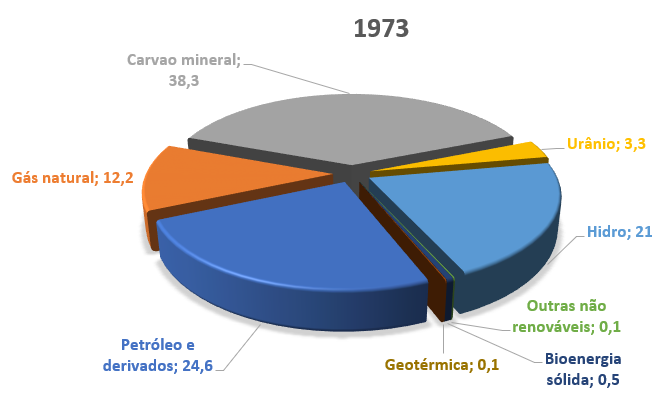
\includegraphics[width=3.125in,height=\textheight]{img/matriz/mundo_73.png}
\caption{Matriz elétrica mundial - 1973, Fonte: MME, Autoria
própria}\label{fig:mundo_73}
}
\end{figure}

\begin{figure}
\hypertarget{fig:mundo_18}{%
\centering
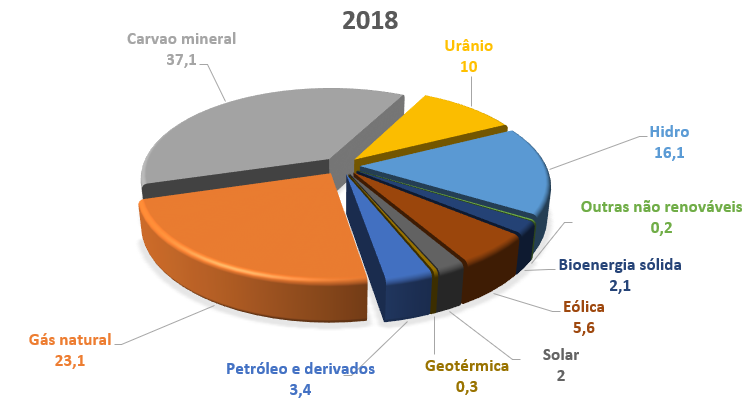
\includegraphics[width=3.125in,height=\textheight]{img/matriz/mundo_18.png}
\caption{Matriz elétrica mundial - 2018, Fonte: MME, Autoria
própria}\label{fig:mundo_18}
}
\end{figure}

A participação do petróleo para geração elétrica também diminuiu ao
redor do globo nos últimos 46 anos, revelando o interesse em fontes
inesgotáveis de energia.

\hypertarget{gerauxe7uxe3o-distribuida}{%
\section{Geração Distribuida}\label{gerauxe7uxe3o-distribuida}}

Nos últimos anos o mundo vem sofrendo mudanças climáticas e outros
desastres socioambientais decorrentes do desenfreado consumismo humano
do ultimo século. Estes desastres mostraram a todos que caso o planeta
não seja bem cuidado os dias do Homem podem estar contados. Tal fato tem
aumentado o receio de autoridades políticas. Com o crescimento desta
inquietação com o meio ambiente, muitas políticas estratégicas vêm sendo
elaboradas com o intuito da preservação do meio ambiente. Essas
políticas fazem parte da estratégia do desenvolvimento sustentável.

No Brasil estas políticas surgiram algum tempo depois, entretanto são
vistas como grandes propulsores para pessoas físicas e jurídicas, as
quais enxergam nestas políticas oportunidades de grandes negócios ou até
mesmo fontes para pequenos retornos e auxílios. Nos últimos vinte anos o
país tem elaborado planos de geração energética sustentável, com planos
de alavancar a nação para mais perto de outros países de
interesse\footnote{http://epe.gov.br/pt/publicacoes-dados-abertos/publicacoes/Plano-Nacional-de-Energia-PNE-2030}.
Redução em impostos e incentivos para produção de energia ``limpa'' como
à base de resíduos ou do vento são grandes exemplos destas políticas
nacionais.\footnote{https://www.camara.leg.br/noticias/561691-comissao-aprova-incentivo-a-geracao-de-energia-a-partir-de-residuos/}

Com tais incentivos, muitas pessoas acabam optado por instalar geradores
em suas residências. A geração própria implica na redução da demanda
energética do fornecedor. Isso faz com que a própria fatura de luz tenha
redução. O investimento em uma fonte de energia local tem também retorno
a longo prazo, devido a fatos como aumento da tarifa repassada pela
ANEEL.

Outrossim, há ocasiões pontuais em que o fornecimento de energia é
impossibilitado, seja por rompimento de cabos entre o consumidor e
distribuidor, interrupções programadas, acidentes no meio do trajeto do
fluxo da energia, ou até mesmo por maus projetos residenciais.\footnote{https://www.cpfl.com.br/energias-sustentaveis/eficiencia-energetica/uso-consciente/falta-de-energia/Paginas/default.aspx}
Como resolução de tais problemas a geração própria acaba sendo muito
favorável, possibilitando ao morador ou empresário o total funcionamento
de seu local de laboro.

Há momentos em que a tarifa de energia sofre alterações, as quais podem
ser ou não previstas. O que usualmente ocorre é o aumento de tarifa para
consumidores residenciais devido ao aumento de trabalho necessário para
fornecimento de eletricidade para as casas, o qual provém de níveis
baixos nos reservatórios das usinas. Como já comentado na
{[}@sec:matriz\_br{]}, como a maior parte da energia depende do setor
hidráulico, em períodos de seca são necessárias mais usinas
trabalhando.\footnote{http://www.aneel.gov.br/bandeiras-tarifarias}
Esses valores de tarifas possuem o nome de ``bandeiras tarifárias''. Um
outro ``aumento'' de tarifa pode ser notado em indústrias, no que
comumente é chamado de ``horário de ponta'', definido como um período de
três horas consecutivas, as quais há um grande acréscimo de energia
demandada para a empresa concessionária, a qual, preservada por leis,
cobra a energia consumida nessa faixa a uma tarifa específica,
logicamente com seu valor mais elevado.\footnote{http://www.mme.gov.br/documents/10584/1985241/Manual\%20de\%20Tarif\%20En\%20El\%20-\%20Procel\_EPP\%20-\%20Agosto-2011.pdf}

Com a produção de energia particular, entretanto, o consumo no período
de ponta pode ser totalmente com base na mesma energia produzida,
fazendo com que o consumo tarifado seja nulo. De mesmo modo, nos
períodos de bandeiras tarifárias vermelhas e amarela, o consumo a ser
pago encaminha-se ao consumo mínimo, o qual é obrigatório ser
pago.\footnote{http://www2.aneel.gov.br/arquivos/PDF/Cartilha\_1p\_atual.pdf}

Não obstante, a geração particular de energia acarreta em uma menor
demanda para a companhia elétrica responsável pela região, o que também
diminui a demanda energética das usinas geradoras de maiores portes. O
que essa diminuição da demanda implica é a dispensabilidade de projetos
para construção de novas usinas. Esses projetos que, como já discutido,
trazem consigo vários percalços.

A partir de 17 de abril de 2012, qualquer consumidor brasileiro pode
produzir sua própria energia, desde que oriunda de fontes renováveis ou
por ``cogeração qualificada''.\footnote{http://www2.aneel.gov.br/cedoc/ren2012482.pdf}
Já em lugares de maior porte, como indústrias e hospitais, pode-se fazer
uso também de geradores a combustão de derivados do petróleo, seja
apenas em horário de ponta ou quando há comprometimento na entrega de
energia. Faz-se importante então um estudo a respeito dessas fontes de
energia.

\hypertarget{gerauxe7uxe3o-a-combustuxe3o}{%
\subsection{Geração a combustão}\label{gerauxe7uxe3o-a-combustuxe3o}}

Os geradores a diesel ou gasolina estão presentes na maioria das
indústrias e hospitais, tanto para atender às necessidades em momentos
que ocorre falta de energia, ou até para uso no período de ponta, com o
intuito de reduzir as contas.

O funcionamento do gerador a combustão baseia-se na lei de Faraday
({[}@eq:leifaraday{]}), onde a variação de campo magnético conduz na
produção de um campo elétrico, também variável. O combustível causa
explosões nos pistões do gerador, os quais são responsáveis para dar
movimento ao rotor.

\[ \oint \vec{E} \cdot d\vec{s} = -\frac{d\phi_B}{dt} \]\{\#eq:leifaraday\}

Essas máquinas contemplam o gerador propriamente dito acoplado com um
motor, o qual é impulsionado a partir de fluidos, como diesel, óleos
pesados, GLP, ou outros derivados do petróleo. Toda a rotação é gerada a
partir da explosão desses fluidos nos pistões do motor (figuras
{[}-@fig:diesel1{]} e {[}-@fig:diesel2{]}).

\begin{figure}
\hypertarget{fig:diesel1}{%
\centering
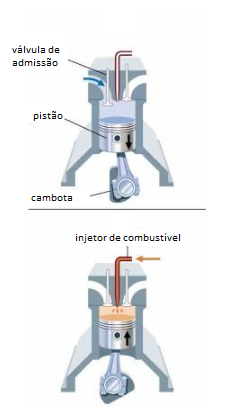
\includegraphics[width=\textwidth,height=3.125in]{img/gerador/motor1.png}
\caption{Admissão (A) e Compressão (B) do ar em motores de
combustão}\label{fig:diesel1}
}
\end{figure}

\begin{figure}
\hypertarget{fig:diesel2}{%
\centering
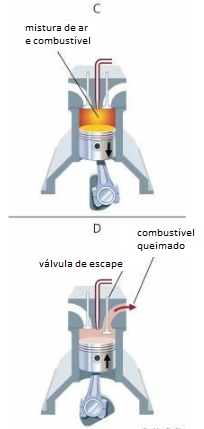
\includegraphics[width=\textwidth,height=3.125in]{img/gerador/motor2.png}
\caption{Expansão (A) e Escape (B) dos gases da combustão motores de
combustão}\label{fig:diesel2}
}
\end{figure}

Em geradores de campo giratório, como o da {[}@fig:rotorgiratório{]}, a
tensão é extraída diretamente dos enrolamentos da armadura
(estator).\footnote{https://static.weg.net/medias/downloadcenter/h68/h68/WEG-curso-dt5-caracter-sticas-e-especifica-o-de-geradores-artigo-tecnico-portugues.pdf}
Com a movimentação do motor, um campo elétrico é induzido na armadura,
donde flui corrente elétrica.

\begin{figure}
\hypertarget{fig:rotorgiratuxf3rio}{%
\centering
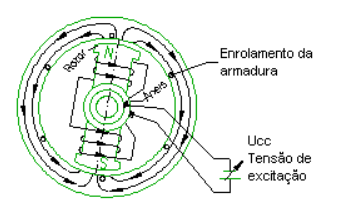
\includegraphics[width=2.08333in,height=\textheight]{img/gerador/geradorarmadurafixa.png}
\caption{Esquema de gerador elemental com armadura fixa -
Fonte:WEG}\label{fig:rotorgiratuxf3rio}
}
\end{figure}

O formato da onda de saída depende do formato que o campo possui em
relação ao tempo, os geradores são construídos com a finalidade de
produzir ondas em formato senoidal.

Como a geração a combustão produz gás carbônico como resultado, a lei
permite o uso dessas máquinas em pequenas faixas ao longo do dia,
objetivando uma menor poluição por parte das empresas.

\hypertarget{gerauxe7uxe3o-euxf3lica}{%
\subsection{Geração eólica}\label{gerauxe7uxe3o-euxf3lica}}

Assim como geradores a combustão, a geração eólica toma como base o
princípio da conversão de energia mecânica em elétrica por meio da lei
de Faraday, a qual testifica a presença de uma força eletromotriz
induzida resultante de uma variação de campo magnético sentido pelo
circuito.\footnote{http://www.ifsc.usp.br/\textasciitilde strontium/Teaching/Material2010-2\%20FFI0106\%20LabFisicaIII/11-LeideInducaodeFaraday.pdf}

A rotação da turbina dos aerogeradores se dá a partir do movimento do
vento, que é captado pelas pás. Devido ao tamanho que as pás captadoras
possuem, sua rotação não atinge os valores necessários para conversões
diretas, então é crucial o uso de caixas de engrenagens, designadas a
multiplicar a velocidade de rotação a ser acoplada ao seu respectivo
gerador ({[}@fig:componentes\_turbina{]}).

\begin{figure}
\hypertarget{fig:componentes_turbina}{%
\centering
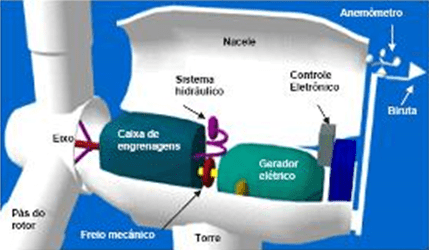
\includegraphics[width=3.125in,height=\textheight]{img/eolico/componente-da-turbina.png}
\caption{Componentes de uma turbina
eólica}\label{fig:componentes_turbina}
}
\end{figure}

O anemômetro é capaz de aferir a intensidade, velocidade e direção do
vento, dando possibilidade de controlar a angulação das pás, para melhor
aproveitamento tanto de rotação quanto da geração.

Mesmo sendo uma fonte de energia renovável e não poluente, a geração
eólica ainda traz consigo algumas adversidades. O ar, ao se chocar com
as pás, provoca ruídos desconfortáveis para a população próxima. Outro
problema a ser citado é o impacto que animais voadores podem causar nas
pás, trazendo danos para a produção e diminuindo a vida útil dos
equipamentos.

Outro ponto observado é a intermitência que os ventos possuem, sendo
provável que em certos momentos de maior demanda não haja vento soprando
suficiente, ou até mesmo em situações de demanda em que não há vento
algum, trazendo para a geração eólica uma inconstância indesejada.

\hypertarget{gerauxe7uxe3o-fotovoltaica}{%
\subsection{Geração fotovoltaica}\label{gerauxe7uxe3o-fotovoltaica}}

Dentre os atuais meios de se produzir energia elétrica, um que está
sempre em voga é a geração fotovoltaica. Essa geração é silenciosa e
abundante. Outro fator que contribui para a geração de energia através
do sol é que a estrela tem uma vida muito longa, e inesgotável,
comparada ao tempo humano na terra. A energia irradiada na Terra chega a
\(9,5.10^4\) terawatts, até 10 mil vezes toda a energia consumida no
planeta\footnote{Grätzel, M. Photoelectrochemical cells. Nature 2001,
  414, 338. {[}CrossRef{]}}.

As células, em trabalho, não produzem gases ou efluentes, fazendo assim
com que o meio ambiente não seja afetado na produção de energia. Este
fator é também outro motivo que aponta a vantagem da energia solar em
relação às outras formas de geração, e um assunto que é discutido
hodiernamente devido à conscientização ambiental a qual muito se fala
atualmente.

\hypertarget{efeito-fotovoltaico}{%
\subsubsection{Efeito fotovoltaico}\label{efeito-fotovoltaico}}

Atualmente, muito se comenta a respeito da energia solar e sua geração
com os painéis e módulos fotovoltaicos. Há muitas pesquisas nesse meio,
com objetivos como tornar a tecnologia mais próxima do público. A
unidade mais simples para a formação dos módulos são as células.

A célula fotovoltaica tem seu funcionamento oriundo do efeito
fotovoltaico. Este fenômeno é mais antigo do que a maioria das pessoas
pensam. Em 1839, Edmond Becquerel percebeu a geração de energia a partir
de luz solar incidindo em placas de latão submersas em um líquido
eletrólito \footnote{Smestad, G. P. Optoelectronics of solar cells, 1a.
  ed., SPIE: Bellingham, 2002.}. Mais tarde, então, Charles Frittts foi
capaz de inventar a primeira bateria de luz solar, feita com base em
selênio\footnote{Komp, R. J. Practical photovoltaics: eletricity from
  solar cells, 3a. ed., aatec publications: Ann Arbor, 2001.}.

Atualmente as células são fabricadas com semicondutores, materiais que
apresentam características intermediárias entre condutores e isolantes.
O elemento mais famoso dentre os semicondutores é o silício. O cristal
de silício puro é mal condutor elétrico, devido ao fato de conter 4
elétrons livres em sua camada de valência. Para que a condução seja
possível, acrescentam-se porcentagens de outros elementos, com a
finalidade de deixar o átomo quase estável. A este processo dá-se o nome
de ``dopagem''.

A partir da dopagem do silício com o arsênio ou o fósforo, elementos que
apresentam 5 elétrons na última camada, formam-se ligações covalentes
entre quatro elétrons, o quinto é propositalmente livre, possibilitando
a passagem de corrente elétrica. Por ser dopado com elétrons a mais, é
nomeado silício tipo N.

A dopagem do silício tipo P é geralmente feita à base de gálio ou boro,
elementos com três elétrons na camada mais distante. Agora são feitas
três ligações covalentes, a quarta ligação é propositalmente ausente, e
também chamada de lacuna({[}@fig:dopagem{]}).

\begin{figure}
\hypertarget{fig:dopagem}{%
\centering
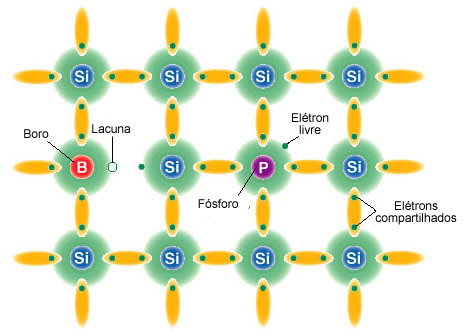
\includegraphics[width=3.125in,height=\textheight]{img/fotovoltaico/dopagem_eletronica.jpg}
\caption{Dopagem Eletrônica, Fonte: Infoescola}\label{fig:dopagem}
}
\end{figure}

A célula fotovoltaica contem as duas dopagens, sendo uma camada fina de
material tipo N e uma camada espessa de material do tipo P, conforme
ilustra a {[}@fig:transversal{]}. Com isso, é gerado um campo elétrico,
também chamado de região PN\footnote{https://www.solenerg.com.br/files/monografia\_cassio.pdf}.
Quando a luz incide na célula, os elétrons recebem energia proveniente
dos fótons. Os elétrons, então excitados, são acelerados e fluem através
da junção. A corrente gerada origina a diferença de potencial entre as
faces P e N.\footnote{https://www.solenerg.com.br/files/monografia\_cassio.pdf}

\begin{figure}
\hypertarget{fig:transversal}{%
\centering
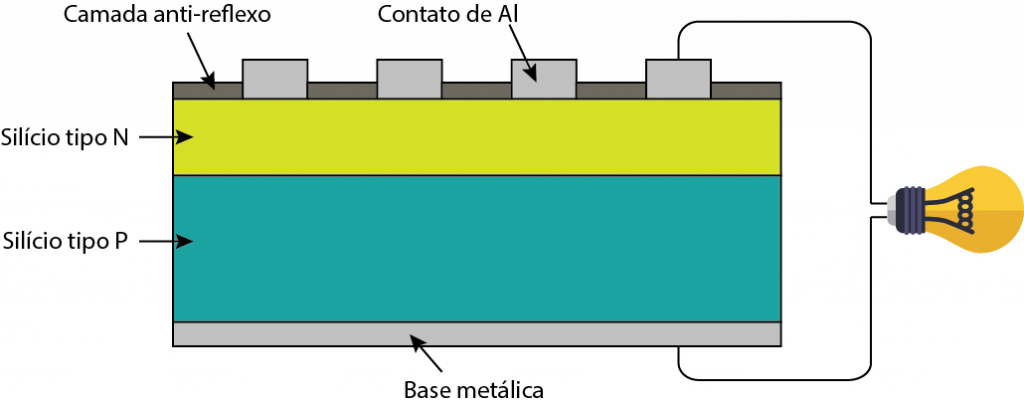
\includegraphics[width=3.125in,height=\textheight]{img/fotovoltaico/placatransversal.png}
\caption{Visão lateral de uma célula
fotovoltaica}\label{fig:transversal}
}
\end{figure}

\hypertarget{cuxe9lulas-fotovoltaicas}{%
\subsubsection{Células fotovoltaicas}\label{cuxe9lulas-fotovoltaicas}}

\textbf{falar dos tipos de paineis monocristalino e policristalino}

\hypertarget{referuxeancias}{%
\section{Referências}\label{referuxeancias}}

\end{document}
%% Comente para remover este item

%% Formatação de páginas de elementos pós-textuais
\postextual%% Não comente esta linha

%% Arquivos de referências
\arquivosdereferencias{%% Arquivos bibtex sem a extensão .bib e separados por vírgula - Não comente esta linha
  ./PosTexto/exemplos-referencias,%% Arquivo de referências - Comente para remover este item
  ./PosTexto/referencias%% Arquivo de referências - Comente para remover este item
}%% Não comente esta linha

%% Glossário
\incluirglossario%% Comente para remover este item

%% Arquivos de apêndices
\begin{arquivosdeapendices}%% Os arquivos de apêndices devem se incluídos neste ambiente - Não comente esta linha
  \partapendices%% Página de início dos apêndices - Comente para remover este item
  %%%% APÊNDICE A
%%
%% Texto ou documento elaborado pelo autor, a fim de complementar sua argumentação, sem prejuízo da unidade nuclear do trabalho.

%% Título e rótulo de apêndice (rótulos não devem conter caracteres especiais, acentuados ou cedilha)
\chapter{Título do Apêndice A com um Texto Muito Longo que Pode Ocupar Mais de uma Linha}\label{cap:apendicea}

Quando houver necessidade pode-se apresentar como apêndice documento(s) auxiliar(es) e/ou complementar(es) como: legislação, estatutos, gráficos, tabelas, etc. Os apêndices são enumerados com letras maiúsculas: \autoref{cap:apendicea}, \autoref{cap:apendiceb}, etc.

No \latex\ apêndices são editados como capítulos. O comando \verb|\appendix| faz com que todos os capítulos seguintes sejam considerados apêndices.

Apêndices complementam o texto principal da tese com informações para leitores com especial interesse no tema, devendo ser considerados leitura opcional, ou seja, o entendimento do texto principal da tese não deve exigir a leitura atenta dos apêndices.

Apêndices usualmente contemplam provas de teoremas, deduções de fórmulas matemáticas, diagramas esquemáticos, gráficos e trechos de código. Quanto a este último, código extenso não deve fazer parte da tese, mesmo como apêndice. O ideal é disponibilizar o código na Internet para os interessados em examiná-lo ou utilizá-lo.

%% Título e rótulo de seção (rótulos não devem conter caracteres especiais, acentuados ou cedilha)
\section{Título da Seção Secundária do Apêndice A}\label{sec:secaoapendicea}

Exemplo de seção secundária em apêndice (\autoref{sec:secaoapendicea} do \autoref{cap:apendicea}).

%% Título e rótulo de seção (rótulos não devem conter caracteres especiais, acentuados ou cedilha)
\subsection{Título da Seção Terciária do Apêndice A}\label{subsec:subsecaoapendicea}

Exemplo de seção terciária em apêndice (\autoref{subsec:subsecaoapendicea} do \autoref{cap:apendicea}).

%% Título e rótulo de seção (rótulos não devem conter caracteres especiais, acentuados ou cedilha)
\subsubsection{Título da seção quaternária do Apêndice A}\label{subsubsec:subsubsecaoapendicea}

Exemplo de seção quaternária em apêndice (\autoref{subsubsec:subsubsecaoapendicea} do \autoref{cap:apendicea}).

%% Título e rótulo de seção (rótulos não devem conter caracteres especiais, acentuados ou cedilha)
\paragraph{Título da seção quinária do Apêndice A}\label{para:paragraphapendicea}

Exemplo de seção quinária em apêndice (\autoref{para:paragraphapendicea} do \autoref{cap:apendicea}).
%% Apêndice - Comente para remover este item
  %%%% APÊNDICE B
%%
%% Texto ou documento elaborado pelo autor, a fim de complementar sua argumentação, sem prejuízo da unidade nuclear do trabalho.

%% Título e rótulo de apêndice (rótulos não devem conter caracteres especiais, acentuados ou cedilha)
\chapter{Orçamentos dos Materiais para Montagem da Bancada Experimental}\label{cap:apendiceb}

\begin{table}[htb]%% Ambiente table
\caption{Orçamento dos materiais n.\textsuperscript{o} 1.}%% Legenda
\label{tab:tab3}%% Rótulo
\begin{tabularx}{\textwidth}{@{\extracolsep{\fill}}lrrr}%% Ambiente tabularx
\toprule
Material              & \multicolumn{1}{c}{Valor (R\$)} & \multicolumn{1}{c}{Quantidade}  & \multicolumn{1}{c}{Total (R\$)} \\ \midrule
Bomba centrífuga      & 2500,00                         & 01                              & 2500,00                         \\
Compressor rotativo   & 3000,00                         & 01                              & 3000,00                         \\
Manômetro diferencial & 450,00                          & 02                              & 900,00                          \\
Termopar              & 370,00                          & 02                              & 740,00                          \\
Válvula de esfera     & 43,00                           & 02                              & 86,00                           \\
Tubulação de PVC      & 10,00                           & 05                              & 50,00                           \\
Conexão de PVC        & 5,00                            & 10                              & 50,00                           \\ \midrule
                      &                                 & \multicolumn{1}{r}{Total (R\$)} & 7326,00                         \\ \bottomrule
\end{tabularx}
\fonte{Autoria própria.}%% Fonte
\end{table}

\begin{table}[htb]%% Ambiente table
\caption{Orçamento dos materiais n.\textsuperscript{o} 2.}%% Legenda
\label{tab:tab4}%% Rótulo
\begin{tabularx}{\textwidth}{@{\extracolsep{\fill}}lrrr}%% Ambiente tabularx
\toprule
Material              & \multicolumn{1}{c}{Valor (R\$)} & \multicolumn{1}{c}{Quantidade}  & \multicolumn{1}{c}{Total (R\$)} \\ \midrule
Bomba centrífuga      & 2700,00                         & 01                              & 2700,00                         \\
Compressor rotativo   & 2950,00                         & 01                              & 2950,00                         \\
Manômetro diferencial & 515,00                          & 02                              & 1030,00                         \\
Termopar              & 350,00                          & 02                              & 700,00                          \\
Válvula de esfera     & 40,00                           & 02                              & 80,00                           \\
Tubulação de PVC      & 8,00                            & 05                              & 40,00                           \\
Conexão de PVC        & 6,00                            & 10                              & 60,00                           \\ \midrule
                      &                                 & \multicolumn{1}{r}{Total (R\$)} & 7560,00                         \\ \bottomrule
\end{tabularx}
\fonte{Autoria própria.}%% Fonte
\end{table}

\begin{table}[htb]%% Ambiente table
\caption{Orçamento dos materiais n.\textsuperscript{o} 3.}%% Legenda
\label{tab:tab5}%% Rótulo
\begin{tabularx}{\textwidth}{@{\extracolsep{\fill}}lrrr}%% Ambiente tabularx
\toprule
Material              & \multicolumn{1}{c}{Valor (R\$)} & \multicolumn{1}{c}{Quantidade}  & \multicolumn{1}{c}{Total (R\$)} \\ \midrule
Bomba centrífuga      & 2600,00                         & 01                              & 2600,00                         \\
Compressor rotativo   & 3100,00                         & 01                              & 3100,00                         \\
Manômetro diferencial & 500,00                          & 02                              & 1000,00                         \\
Termopar              & 400,00                          & 02                              & 800,00                          \\
Válvula de esfera     & 45,00                           & 02                              & 90,00                           \\
Tubulação de PVC      & 12,00                           & 05                              & 60,00                           \\
Conexão de PVC        & 5,00                            & 10                              & 50,00                           \\ \midrule
                      &                                 & \multicolumn{1}{r}{Total (R\$)} & 7700,00                         \\ \bottomrule
\end{tabularx}
\fonte{Autoria própria.}%% Fonte
\end{table}
%% Apêndice - Comente para remover este item
\end{arquivosdeapendices}%% Não comente esta linha

%% Arquivos de anexos
\begin{arquivosdeanexos}%% Os arquivos de anexos devem se incluídos neste ambiente - Não comente esta linha
  \partanexos%% Página de início dos anexos - Comente para remover este item
  %%%% ANEXO A
%%
%% Texto ou documento não elaborado pelo autor, que serve de fundamentação, comprovação e ilustração.

%% Título e rótulo de anexo (rótulos não devem conter caracteres especiais, acentuados ou cedilha)
\chapter{Direitos Autorais - Lei N\texorpdfstring{.\textsuperscript{o}}{o.} 9.610, de 19 de Fevereiro de 1998: Disposições Preliminares}\label{cap:anexoa}

\centerline{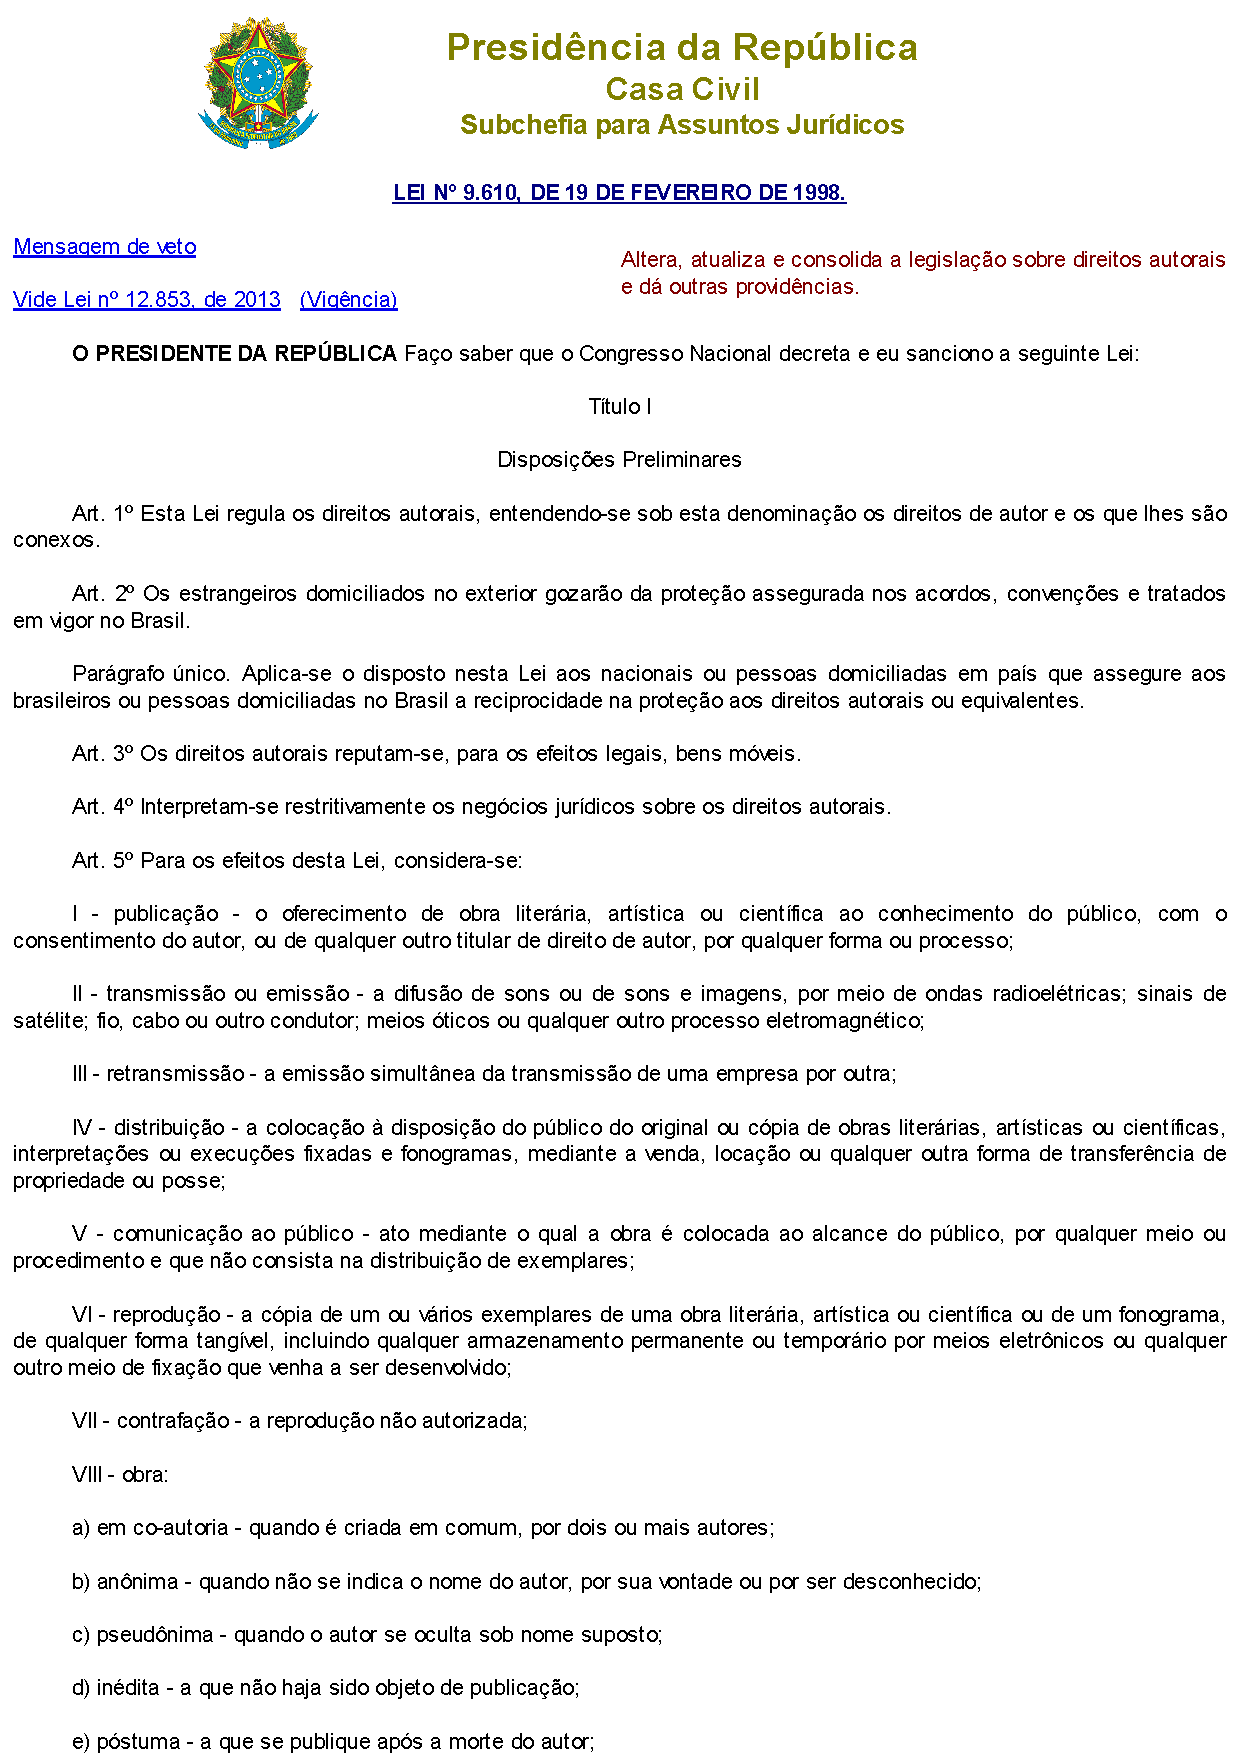
\includegraphics[width=\textwidth]{./PosTexto/Ilustracoes/lei-n9610-p1}}%% Imagem (Dimensões e localização)

\centerline{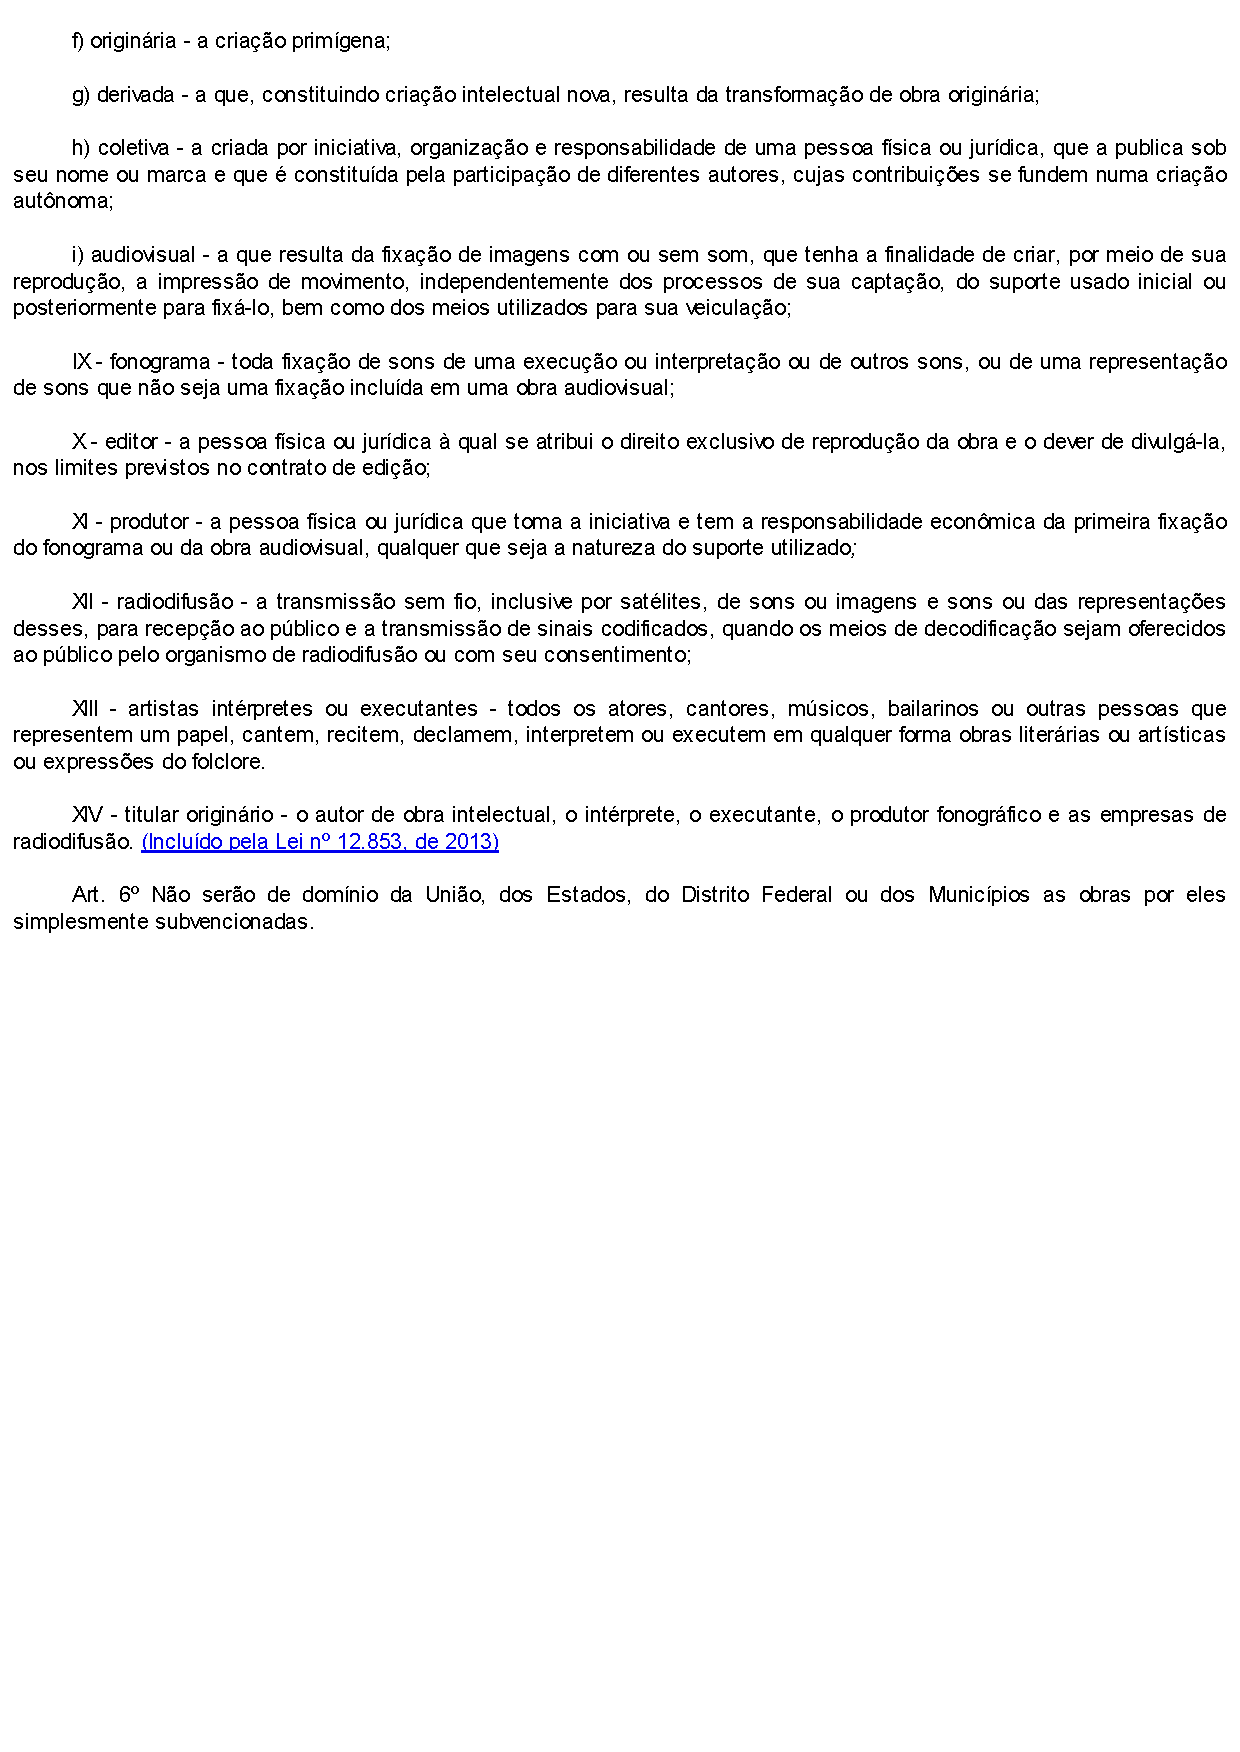
\includegraphics[width=\textwidth]{./PosTexto/Ilustracoes/lei-n9610-p2}}%% Imagem (Dimensões e localização)
%% Anexo - Comente para remover este item
  %%%% ANEXO B
%%
%% Texto ou documento não elaborado pelo autor, que serve de fundamentação, comprovação e ilustração.

%% Título e rótulo de anexo (rótulos não devem conter caracteres especiais, acentuados ou cedilha)
\chapter{Capa do Livro: Normas para Elaboração de Trabalhos Acadêmicos}\label{cap:anexob}

\begin{figure}[htb]%% Ambiente figure
\captionsetup{width=0.9\textwidth}%% Largura da legenda
\caption{Capa do livro: Normas para Elaboração de Trabalhos Acadêmicos.}%% Legenda
\label{fig:capadolivro}%% Rótulo
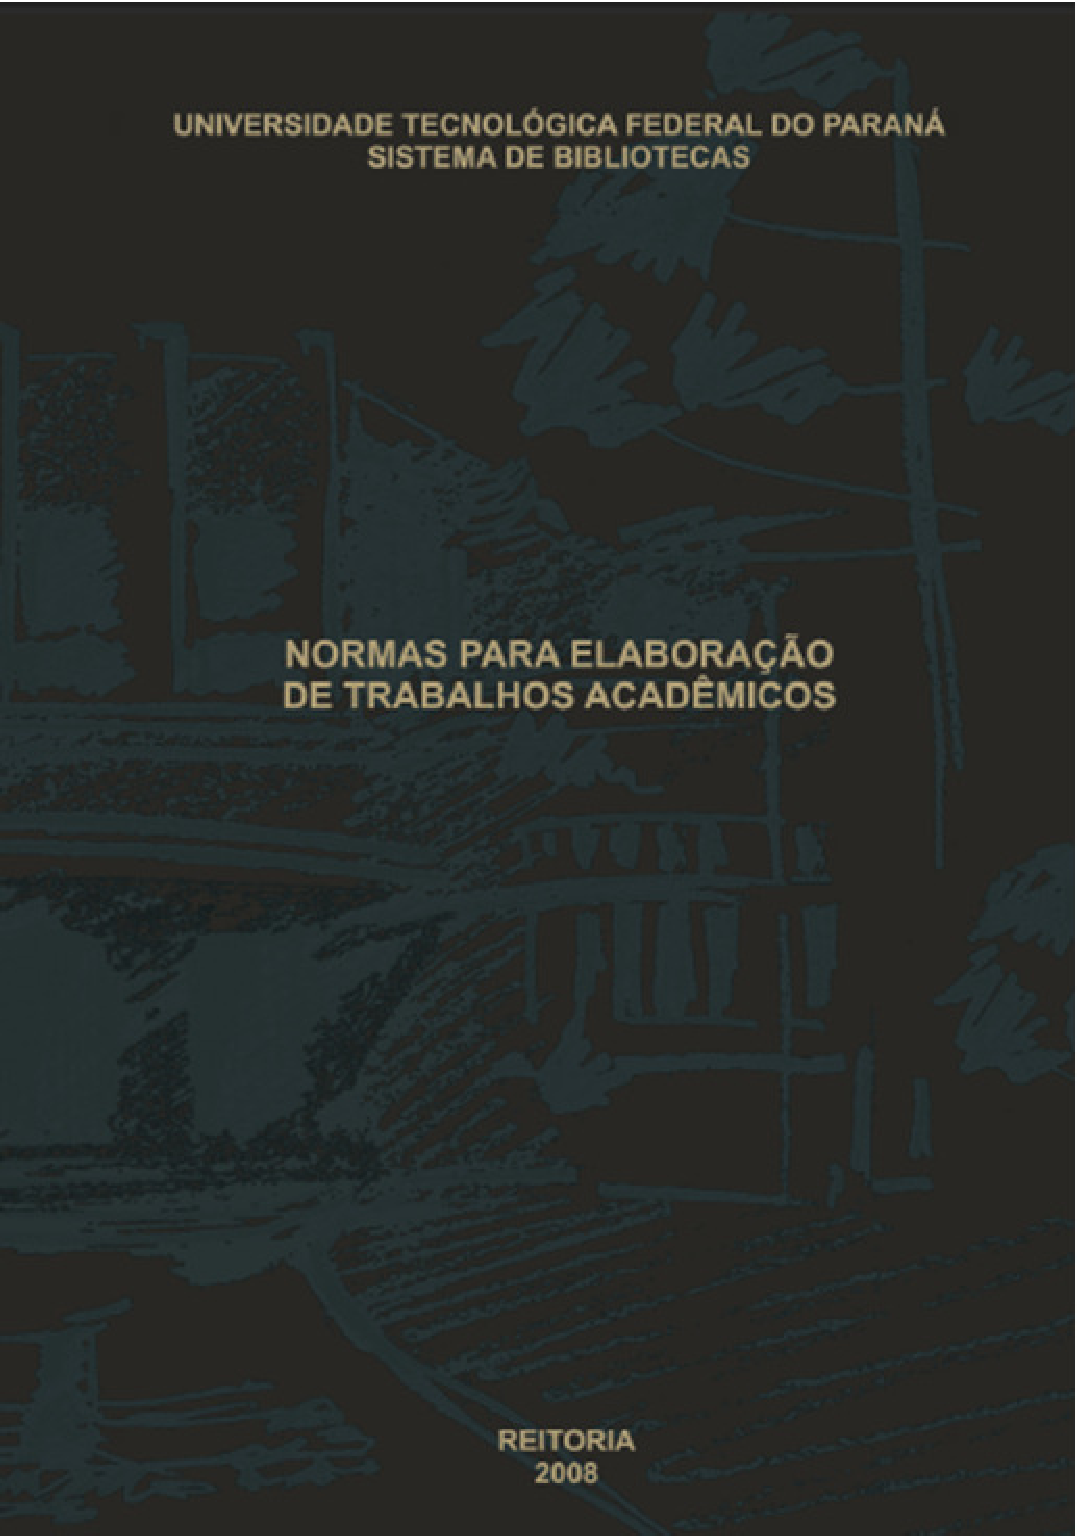
\includegraphics[width=0.9\textwidth]{./PosTexto/Ilustracoes/capa-livro}%% Dimensões e localização
\fonte{\citet{UTFPR2008}.}%% Fonte
\end{figure}
%% Anexo - Comente para remover este item
\end{arquivosdeanexos}%% Não comente esta linha

%% Índice
\incluirindice%% Comente para remover este item

%% Fim do documento
\end{document}%% Não comente esta linha
